\chapter*{About}
\addcontentsline{toc}{chapter}{Preface}

\noindent
This is the manual for the Stan programming language and algorithms.

The Stan project comprises a domain-specific language for
probabilistic programming, a differentiable mathematics and
probability library, algorithms for Bayesian posterior inference and
posterior analysis, along with interfaces and analysis tools in all of
the popular data analysis languages.


\section*{Interfaces and Platforms}

Stan runs under Windows, Mac OS X, and Linux.

Stan uses a domain-specific programming language that is portable
across data anlsysi languages.  Stan has interfaces for R, Python,
Julia, MATLAB, Mathematica, Stata, and the command line, as well
as an alternative language interface in Scala.  See the web
site (link below) for links and getting started instructions.

\section*{Web Site}

The official resource for all things related to Stan is the web site:
%
\begin{quote}
\url{http://mc-stan.org}
\end{quote}
%
The web site links to all of the packages comprising Stan for both
users and developers.  This is the place to get started with Stan.
Find the interface in the language you want to use and follow the
download, installation, and getting started instructions.  


\section*{GitHub Organization}

Stan's source code and much of the developer process is hosted on
GitHub.  Stan's organization is:
%
\begin{quote}
\url{http://https://github.com/stan-dev}
\end{quote}
%
Each package has its own repository within the \code{stan-dev}
organization.  The web site is also hosted and managed through GitHub.
This is the place to peruse the source code, request features, and
report bugs.  Much of the ongoing design discussion is hosted on the
GitHub Wiki.


\section*{Forums}

Stan hosts message boards for discussing all things
related to Stan.  
%
\begin{quote}
\url{http://discourse.mc-stan.org}
\end{quote}
%
This is the place to ask questions about Stan, including modeling,
programming, and installation.


\section*{Licensing}

The core C++ code underlying Stan, including the math library,
language, and inference algorithms, is licensed under the BSD 3-clause
licensed as detailed in each repository and on the web site along
with the distribution links.


\section*{Acknowledgements}

The Stan project could not exist without the generous grant
funding of many grant agencies to the participants in the project.
For more details of direct funding for the project, see the web site
and project pages of the Stan developers.

The Stan project could also not exist without the generous
contributions of its users in reporting and in many cases fixing bugs
in the code and its documentation.  We used to try to list all of
those who contributed patches and bug reports for the manual here, but
when that number passed into the hundreds, it became too difficult to
manage reliably.  Instead, we will defer to GitHub (link above), where
all contributions to the project are made and tracked.

Finally, we should all thank the Stan developers, without whom this
project could not exist.  We used to try and list the developers here,
but like the bug reporters, once the list grew into the dozens, it
became difficult to track.  Instead, we will defer to the Stan web
page and GitHub itself for a list of core developers and all developer
contributions respectively.

\vfill
\begin{center}
\hfill
\begin{minipage}[b]{2in}
  \footnotesize {\it Stanislaw Ulam, namesake of Stan and co-inventor
    of Monte Carlo methods \citep{MetropolisUlam:1949}, shown here
    holding the Fermiac, Enrico Fermi's physical Monte Carlo simulator
    for neutron diffusion.}
  \\[3pt] \mbox{ } \hfill
  {\scriptsize Image from \citep{Giesler:2000}.}
\end{minipage} \ \ \ \ \
\begin{minipage}[b]{1.5in} \mbox{ } \hfill
  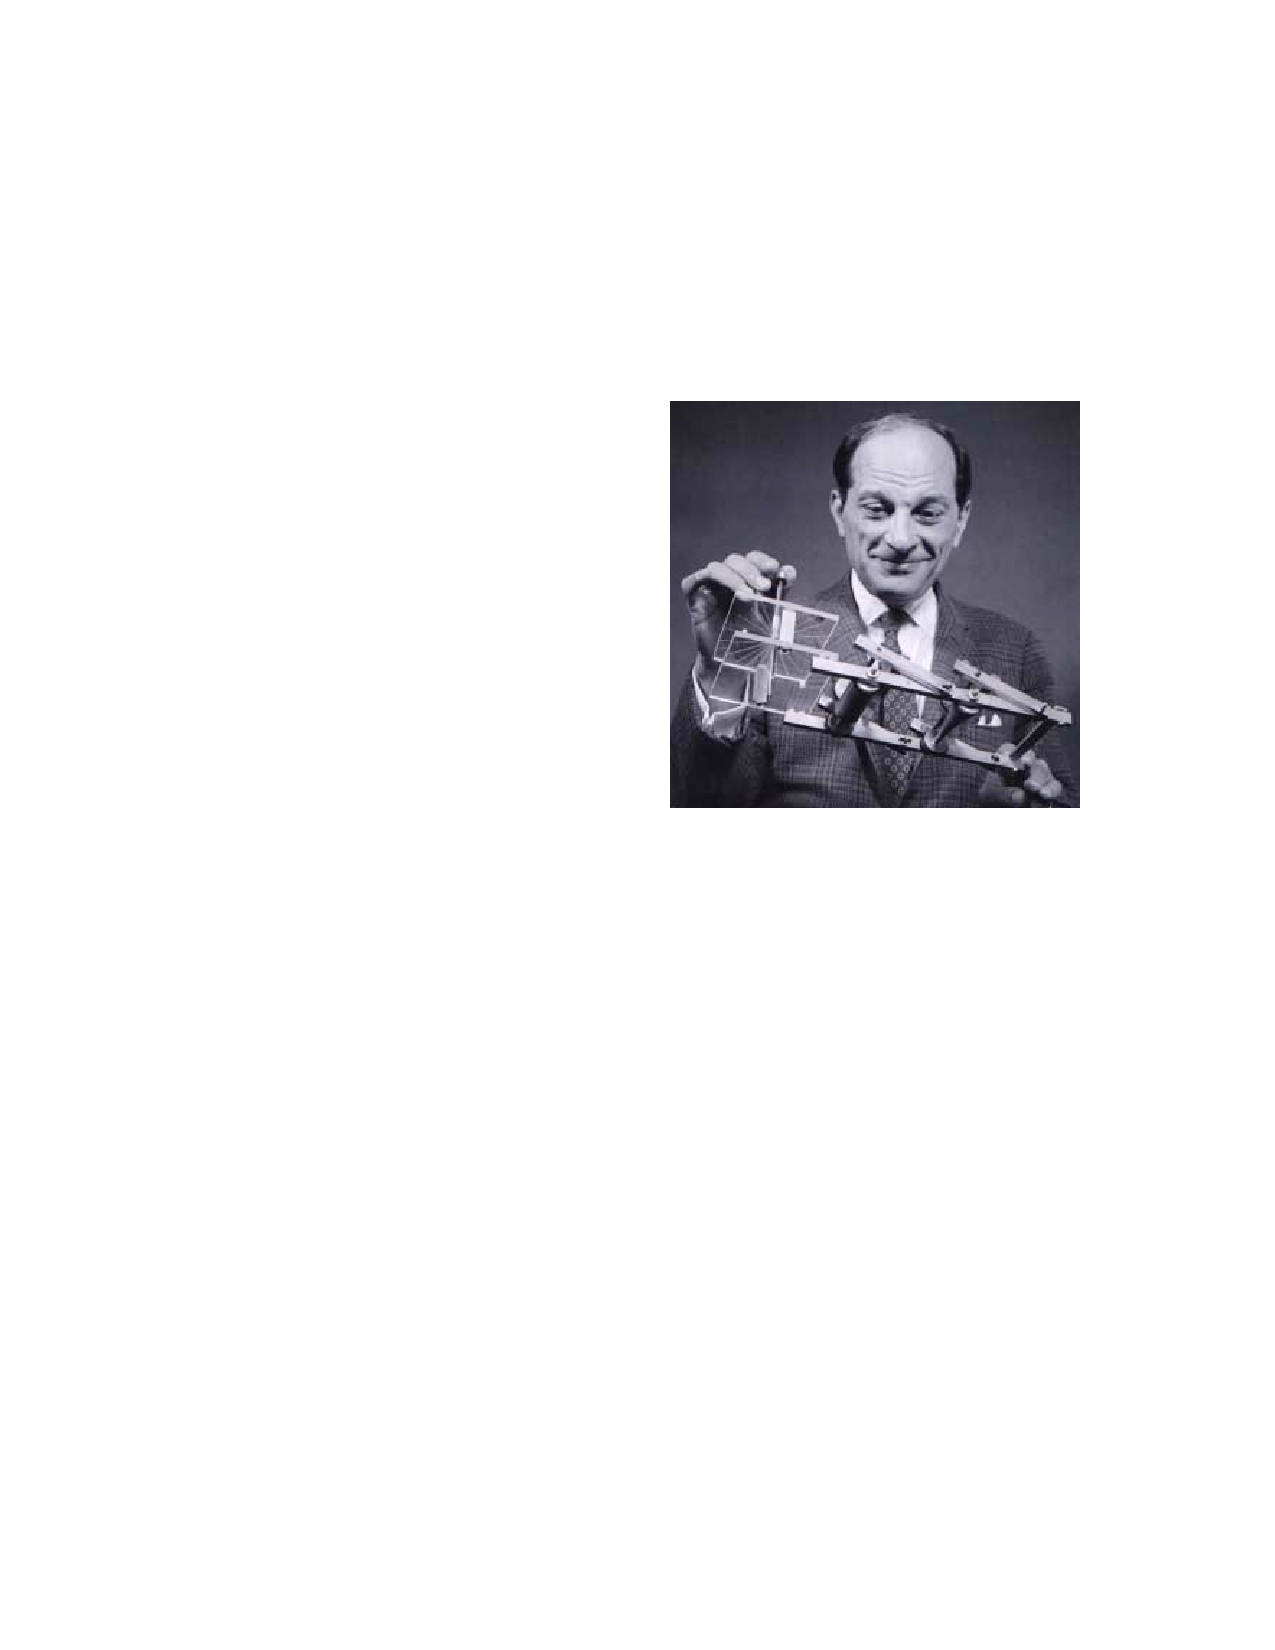
\includegraphics[width=1.5in]{img/ulam-fermiac.pdf}
\end{minipage}
\end{center}
